\subsection{Level3.1: パラメータのチューニング}
\subsubsection{最適なパラメータを探すためのアプローチ}
指定された条件下において学習が効率良く行われるパラメータの組み合わせを探
すため,3つのパラメータ ETA, ALPHA, HIDDEN を一つづつ変動させ,
総当たりすることで最適なパラメータを探索した。
具体的には 
ETA を 0.00 - 1.98 までの 0.01 刻み,
ALPHA を 0.00 - 1.98 までの 0.01 刻み,
HIDDEN を 1 - 15 までの 1 刻み 
の計 594015 回 で変動させていき,探索を行った。\\
 探索を行った各パラメータによる実行結果より,最もiteration が低い
パラメータ群を最適な組み合わせとして決定するという方法をとった。//
 また,seed値については,各seed値についても総当たりを行いたいが,
それでは,実行時間がレポート提出期間内に終わらないため,今回の
総当たりはseed値を1000 に固定して行った。

\subsubsection{実行結果}
seed値 1000 において パラメータを総当たりで探索した結果,iteration が最低となった
パラメータは ETA 1.83 ALPHA 0.73 HIDDEN 15 であった。\\
このパラメータを用いて各seed値で実行した際の学習収束回数を以下の図\ref{table:level3}
に示す。

\begin{table}[htb]
 \begin{center}
  \caption{階層型NNによる文字認識問題の学習に要した回数}
  \label{table:level3}
  \begin{tabular}[htb]{r|l} \hline
   シード値 & 収束した回数 \\ \hline \hline
   100 & 173 \\ \hline
   200 & 258 \\ \hline
   300 & 213 \\ \hline
   400 & 250 \\ \hline
   500 & 369 \\ \hline
   600 & 196 \\ \hline
   700 & 121 \\ \hline
   800 & 204 \\ \hline
   900 & 1325 \\ \hline
   1000 & 69 \\ \hline \hline
   10試行の平均値 & 317.8 \\ \hline
  \end{tabular}
 \end{center}
\end{table}

以下の図\ref{fig:level3-1}に求めたパラメータを用いた際の学習曲線を示す。
\begin{figure}[H]
 \begin{center}
  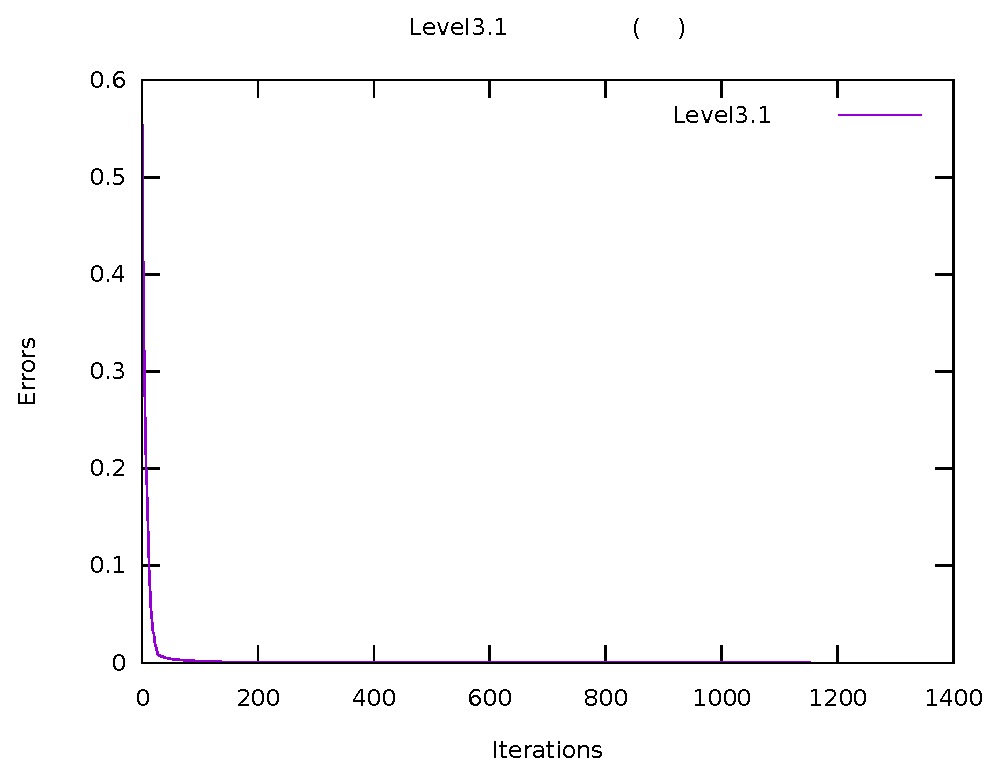
\includegraphics[width=10.0cm]{figs/level3_1/averageGraph.eps}
  \caption{重みを更新する様子(平均値)}
  \label{fig:level3-1}
 \end{center}
\end{figure}

上記の図\ref{fig:level3-1}では,変化が見えづらいため変化の著しい iteration 50までの
図を下図\ref{fig:level3-1-2}に示す。
\begin{figure}[H]
 \begin{center}
  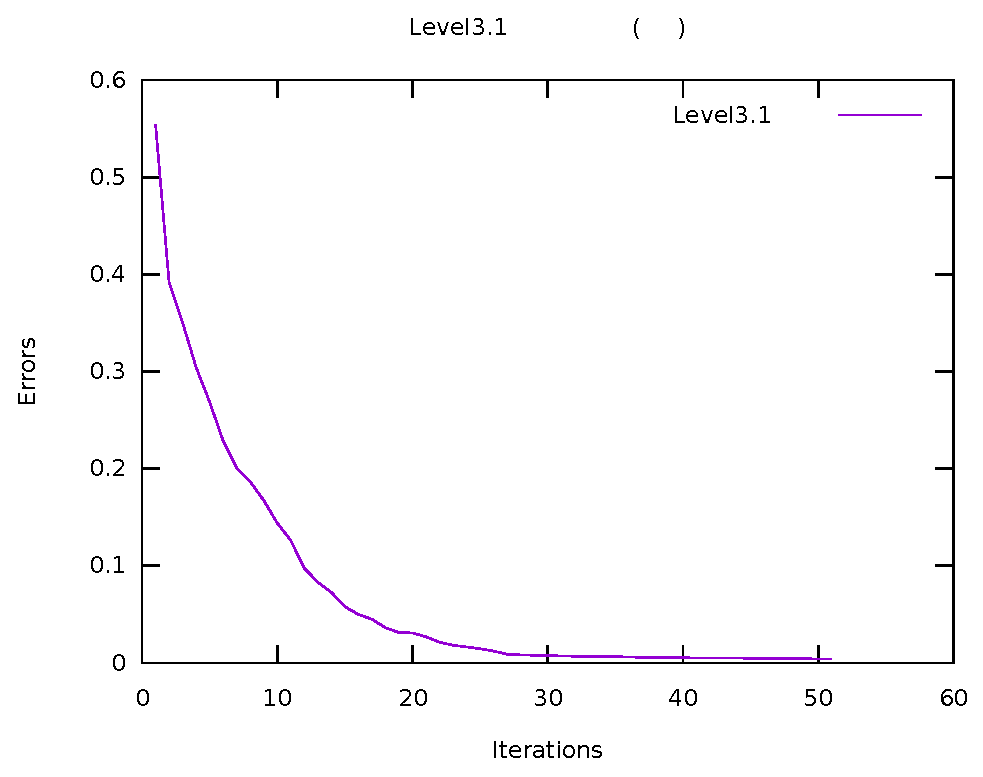
\includegraphics[width=10.0cm]{figs/level3_1/averageGraph2.eps}
  \caption{重みを更新する様子(平均値)拡大図}
  \label{fig:level3-1-2}
 \end{center}
\end{figure}

\subsubsection{考察}
今回seed値を固定してパラメータの組み合わせの総当たりを調べたのには,
seed値を可変にして総当たりを行うと膨大な時間がかかるという理由と,
seed値はニューロンへの入力の重要度の初期値を決定するために用いるだけであるから,
重要度の初期値がどうであれ,ETA,ALPHA,HIDDEN のパラメータが最適な組み合わせであれば,
学習に影響はないであろうという大雑把な予測からであった。しかし,今回の実験結果
(図\ref{table:level3})を見ると,seed値1000 と seed値900 の学習収束回数間には
1200 回以上の差がある。
 このことから,ニューロンへの入力信号の重要度も学習の収束回数へ影響を及ぼし,
"最適なパラメータの組み合わせ"にはETA,ALPHA,HIDDEN の3つの他にseed値 も含まれた
ものであったと考察する。
